\clearpage

\section{Vergleich Mesh Netzwerke}\label{sec:VergleichMeshNetzwerke}

\todo[inline]{Raffi}

\todo[inline]{Verweis auf das Paper. Die wichtigsten Resultate und Erkenntnisse sind im Paper zusammengefasst.}
\todo[inline]{Interpretation und Diskussion der Messresultate. Qualitativer Vergleich der drei Mesh Protokolle. Kritische Betrachtung der Resultate. Gibt es einschneidende Unterschiede zwischen den 3 Netzen die zu einem verfälschten Resultat geführt haben?}

Der Vergleich der Mesh-Netzwerke basiert auf den Messergebnissen der Messreihen, welche in Abschnitt \ref{subsec:Messreihe} erwähnt wurden. Eine Messung unterscheidet sich durch die unterschiedlichen Messparameter, sowie durch den Messaufbau (Wohnung / Labor / Haus). Um einen Vergleich ziehen zu können, wird daher nach diesen beiden Hauptmerkmalen unterschieden.

\subsection{Vergleich Messreihen}\label{subsec:VergleichMessreihen}

Dieser Vergleich bezieht sich auf die selbe Testumgebung, jedoch mit unterschiedlichen Messreihen. Als Referenz wurde die Umgebung des Labors ausgewählt, da Messergebnisse aller Messreihen vorliegen (siehe Anhang \ref{app:MessprotokolleMeshBenchmark}). Im Anschluss soll gezeigt werden wie sich die einzelnen Mesh-Netzwerke bei veränderten Messreihen verändern. \\

Zusammengefasst lassen sich die Messreihen folgendermassen unterscheiden. 

\begin{itemize}
	\item \textbf{\textit{Payload}} Die Payload wurde zwischen den Messreihen 1-3, 2-4 und 7-8 von 8 Byte auf 32 Byte, resp. 50 Byte erhöht.
	\item \textbf{\textit{Traffic Generation Mode}} Wurde zwischen den Messreihen 1-2 und 3-4 von Random auf Sequentiel geändert.
	\item \textbf{\textit{Message Dichte}} Wurde zwischen den Messreihen 2-7 und 4-8 von 2.5 M/s auf 0.33 M/s gesenkt (Messages/Sekunde).
	\item \textbf{\textit{Disturbance}} Wurde zwischen den Messreihen 2-6 eingeschaltet.
\end{itemize}

\subsubsection{Latenzzeit}\label{subsec:VergleichLatenzzeitMessreihen}

\begin{figure}[H]
	\centering
	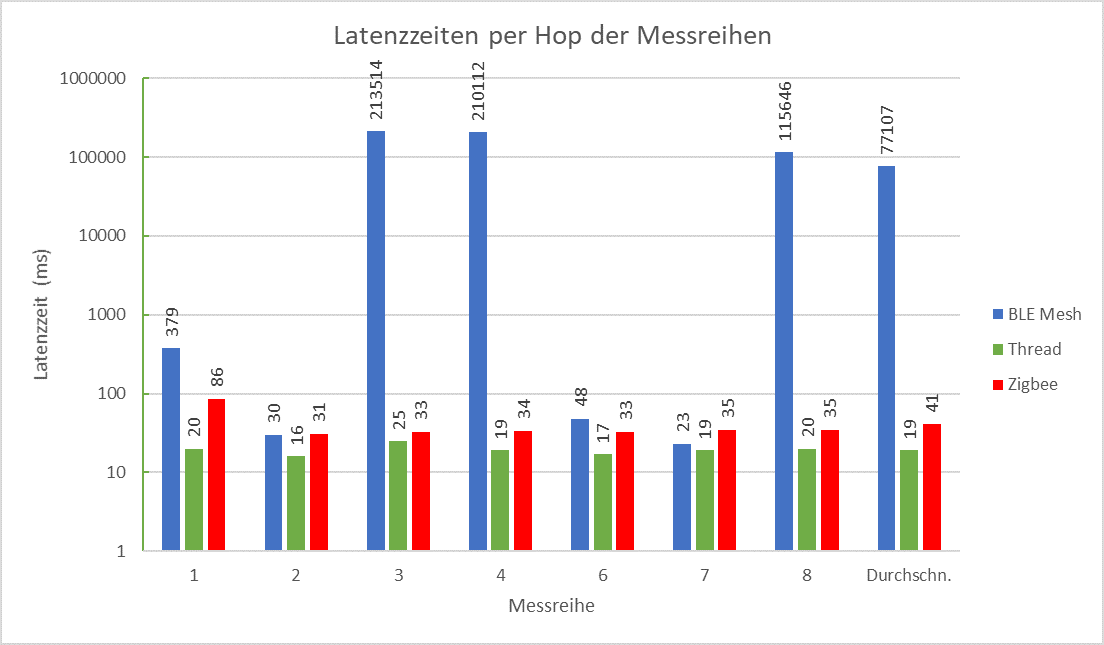
\includegraphics[width=1.0\textwidth]{Latenzzeiten_per_Hop_Messreihen.png}
	\caption{Durchschnittliche Latenzzeit per Hop der einzelnen Messreihen im Vergleich}\label{fig:Latenzzeiten_per_Hop_Messreihen}
\end{figure}

Durch die in Abbildung \ref{fig:Latenzzeiten_per_Hop_Messreihen} dargestellten Latenzzeiten wird ersichtlich das Bluetooth-Mesh am anfälligsten auf ein erhöhen der Payload reagiert. Eine detaillierte Analyse zu diesem Phänomen wird in Abschnitt \ref{subsec:Bluetooth_Mesh} durchgeführt. Die Verzögerung bleibt bei Zigbee und Thread trotz Erhöhung der Paketlänge stabil. \\

Ein Änderung des Traffic Generation Mode von Random auf Sequentiel bewirkt bei Bleutooth-Mesh eine drastische Abnahme der Latenz. Bei Zigbee ist zwischen der Messreihe 1 und 2 ebenfalls eine Abnahme zu verzeichnen, welche jedoch nicht zwischen der Reihe 3 und 4 feststellbar ist. Somit muss ein anderer Einfluss für die Abnahme verantwortlich sein (in Abschnitt \ref{subsec:Zigbee} untersucht). Die Änderung des Traffic Generation Mode wirkt bei Thread ebenfalls zu einer Verbesserung der Latenz.\\

 Das senken der Message Dichte führt bei Bluetooth-Mesh zu einer markanten Abnahme der Latenz. Bei Thread und Zigbee bleibt die Latenz nahezu identisch. \\
 
 Das einbringen von Störungen hat lediglich bei Bluetooth-Mesh einen negativen Einfluss, wodurch sich die Latenzzeit erhöht. 

\subsubsection{Durchsatz}\label{subsec:VergleichDurchsatzMessreihen}


\begin{figure}[H]
	\centering
	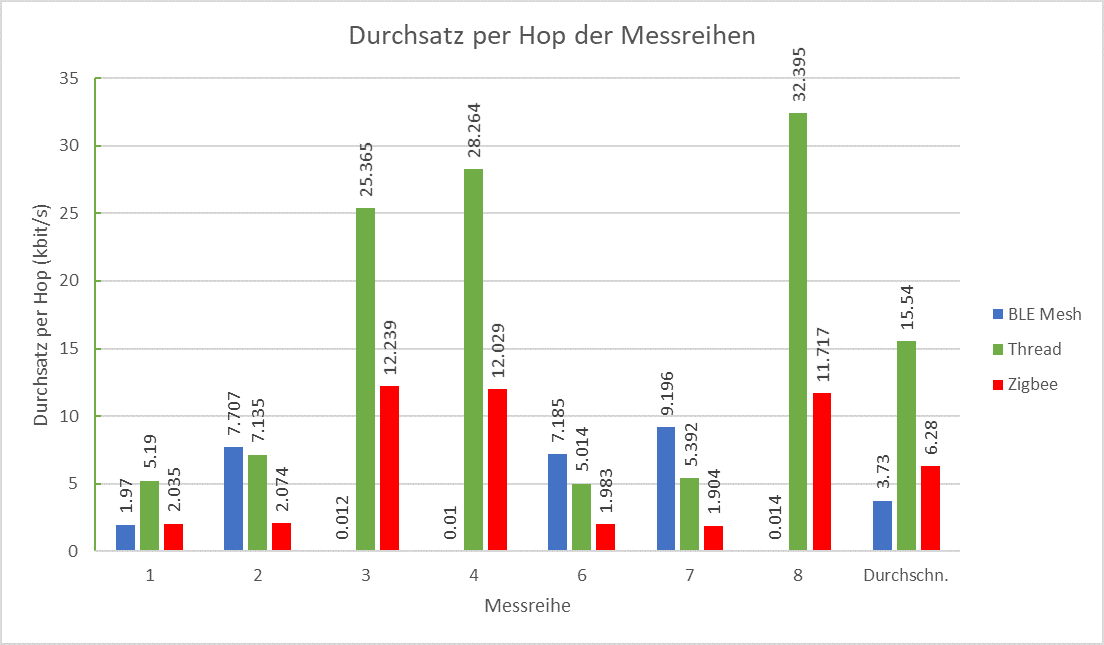
\includegraphics[width=1.0\textwidth]{Durchsatz_per_Hop_Messreihen.png}
	\caption{Durchschnittlicher Durchsatz per Hop der einzelnen Messreihen im Vergleich}\label{fig:Durchsätze_per_Hop_Messreihen}
\end{figure}


Durch die in Abbildung \ref{fig:Durchsätze_per_Hop_Messreihen} dargestellten Durchsätze wird ersichtlich das Bluetooth-Mesh am anfälligsten auf ein erhöhen der Payload reagiert. Wie bereits in Abschnitt \ref{subsec:VergleichLatenzzeitMessreihen} dargelegt wird eine detaillierte Analyse zu diesem Phänomen in Abschnitt \ref{subsec:Bluetooth_Mesh} durchgeführt. Der Durchsatz steigt bei Zigbee und Thread durch die Erhöhung der Paketlänge stark an. Dies wird in Abschnitt \ref{subsec:Thread} für Thread und Abschnitt \ref{subsec:Zigbee} für Zigbee genauer Untersucht. \\

Ein Änderung des Traffic Generation Mode von Random auf Sequentiel bewirkt bei Bleutooth-Mesh eine drastische Abnahme der Latenz. Bei Zigbee ist zwischen der Messreihe 1 und 2 ebenfalls eine Abnahme zu verzeichnen, welche jedoch nicht zwischen der Reihe 3 und 4 feststellbar ist. Somit muss ein anderer Einfluss für die Abnahme verantwortlich sein (in Abschnitt \ref{subsec:Zigbee} untersucht). Die Änderung des Traffic Generation Mode wirkt bei Thread ebenfalls zu einer Verbesserung der Latenz.\\

Das senken der Message Dichte führt bei Bluetooth-Mesh zu einer markanten Abnahme der Latenz. Bei Thread und Zigbee bleibt die Latenz nahezu identisch. \\

Das einbringen von Störungen hat lediglich bei Bluetooth-Mesh einen negativen Einfluss, wodurch sich die Latenzzeit erhöht. 

\subsubsection{Paketverlust}\label{subsec:VergleichPaketverlustMessreihen}


\begin{figure}[H]
	\centering
	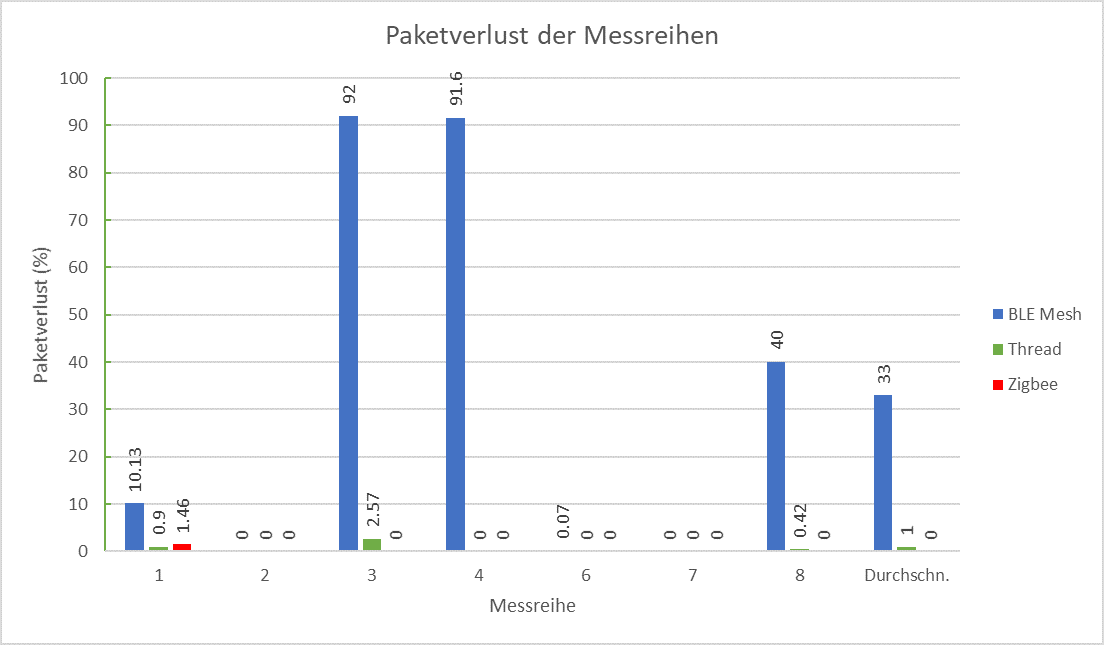
\includegraphics[width=1.0\textwidth]{Paketverlust_Messreihen.png}
	\caption{Durchschnittlicher Paketverlust der einzelnen Messreihen im Vergleich}\label{fig:PaketverlusteMessreihen}
\end{figure}

\subsubsection{Energieverbrauch}\label{subsec:VergleichEnergieverbrauchMessreihen}


\begin{figure}[H]
	\centering
	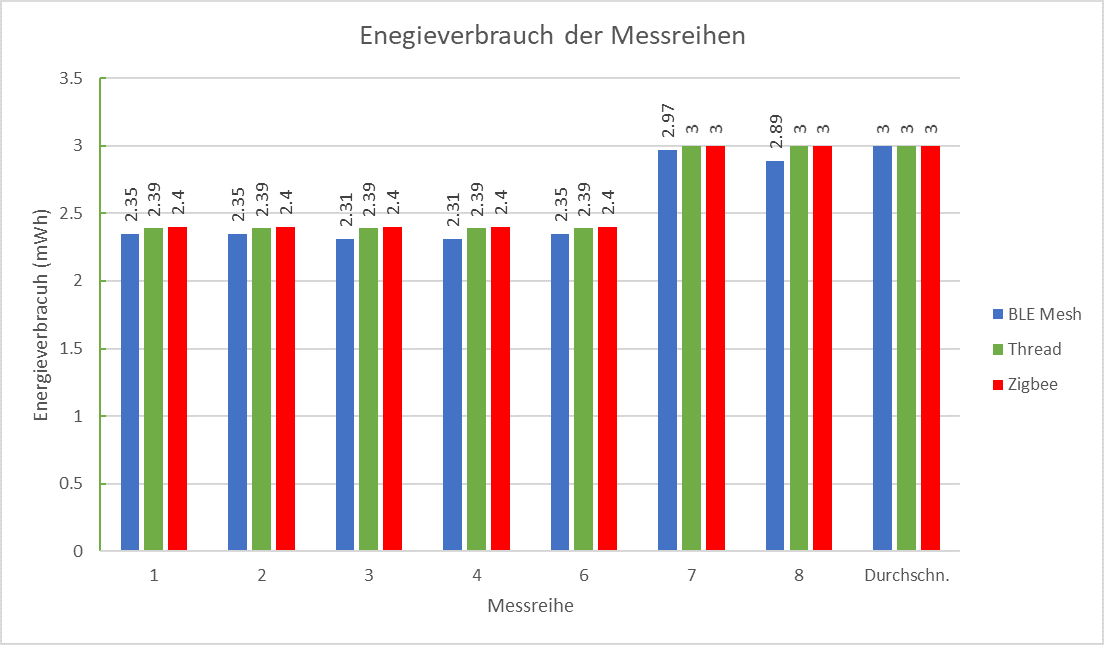
\includegraphics[width=1.0\textwidth]{Energieverbrauch_Messreihen.png}
	\caption{Durchschnittlicher Energiebedarf der einzelnen Messreihen im Vergleich}\label{fig:PaketverlusteMessreihen}
\end{figure}



\subsection{Vergleich Testumgebungen}\label{subsec:VergleichTestumgebungen}

Mithilfe der Unterschiedlichen Testumgebungen wird e

\todo[inline]{Vergleich der drei Netze anhand von spezifischen Merkmalen. Welches Protokoll ist für welche Anwendung geeignet? Wo ist welches Protokoll nicht geeignet?}


\subsubsection{Latenzzeit}\label{subsec:VergleichLatenzzeitTestumgebungen}


\begin{figure}[H]
	\centering
	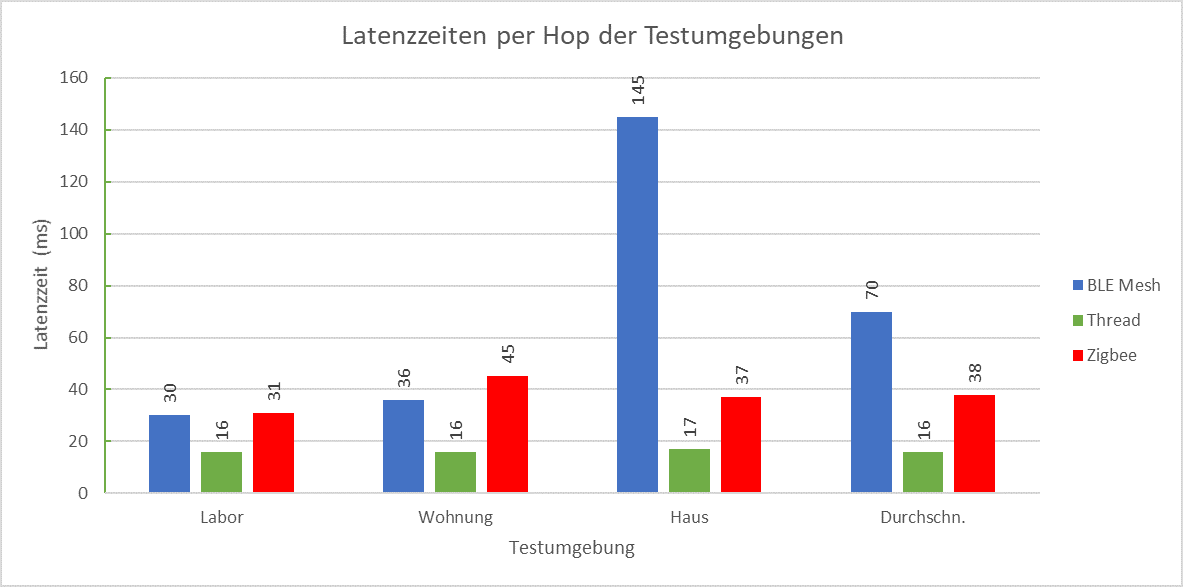
\includegraphics[width=1.0\textwidth]{Latenzzeiten_per_Hop_Testumgebungen.png}
	\caption{Durchschnittliche Latenzzeit per Hop der einzelnen Testumgebungen im Vergleich}\label{fig:Latenzzeiten_per_Hop_Testumgebungen}
\end{figure}

\subsubsection{Durchsatz}\label{subsec:VergleichDurchsatzTestumgebungen}


\begin{figure}[H]
	\centering
	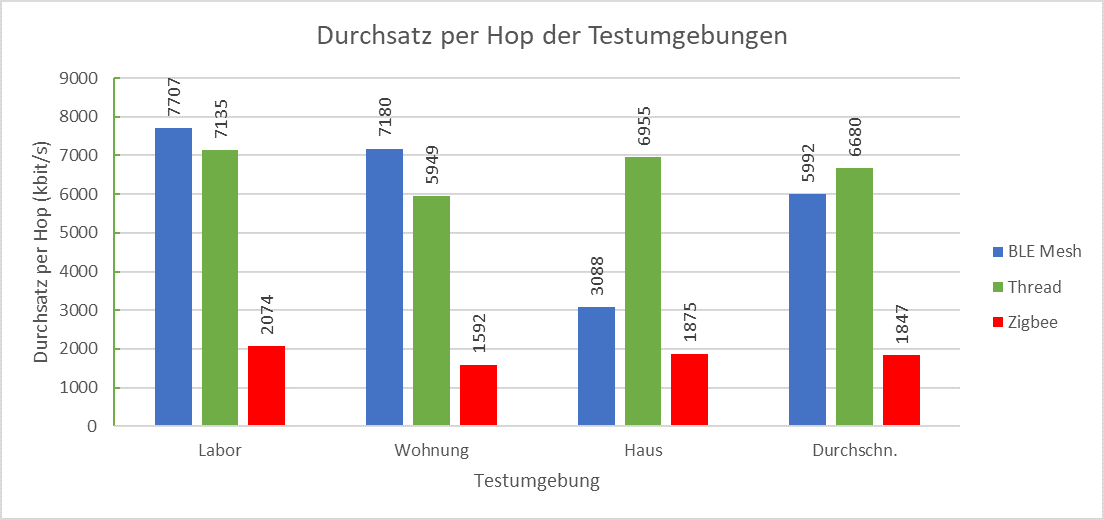
\includegraphics[width=1.0\textwidth]{Durchsatz_per_Hop_Testumgebungen.png}
	\caption{Durchschnittlicher Durchsatz per Hop der einzelnen Testumgebungen im Vergleich}\label{fig:Durchsätze_per_Hop_Testumgebungen}
\end{figure}

\subsubsection{Paketverlust}\label{subsec:VergleichPaketverlustTestumgebungen}


\begin{figure}[H]
	\centering
	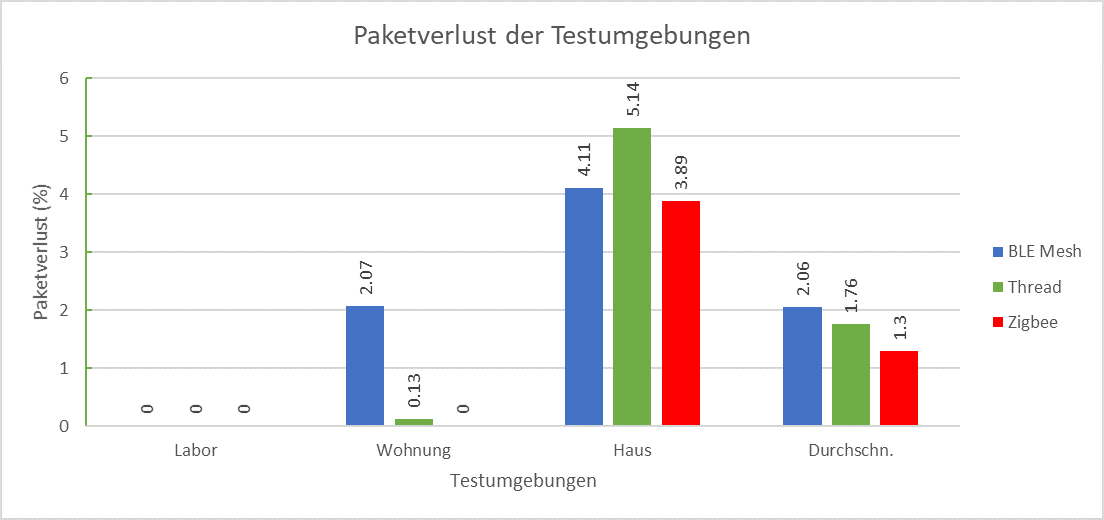
\includegraphics[width=1.0\textwidth]{Paketverlust_Testumgebungen.png}
	\caption{Durchschnittlicher Paketverlust der einzelnen Testumgebungen im Vergleich}\label{fig:PaketverlusteTestumgebungen}
\end{figure}



\subsection{Fazit}\label{subsec:Fazit}
\todo[inline]{Finale Interpretation der Resultate. Welches Protokoll ist das Beste?}

\todo[inline]{Pro / COntra eigene Einschätzung des Stacks... z.B. Thread optimal für Homeautomation.. eher nicht geeiget für Smart Agriculture}

\subsection{Thread}\label{subsec:Thread}

\todo[inline]{Rouben}

\todo[inline]{Erhöhung der Paketlänge führt zu steigerung des Durchsatzes -> Paylod von 50 Byte reicht aus um innerhalb eines Pakets versendet zu werden. }

\subsection{Zigbee}\label{subsec:Zigbee}

\todo[inline]{Cyrill}

\todo[inline]{Warum ist die Latenzeit unabhängig vom Traffic Generation Mode zu beginn kleiner als Zuvor? -> Einrouten des Protocolls zu beginn noch nicht abgeschlossen)}

\todo[inline]{Erhöhung der Paketlänge führt zu steigerung des Durchsatzes -> Paylod von 50 Byte reicht aus um innerhalb eines Pakets versendet zu werden. }

\subsection{Bluetooth Mesh}\label{subsec:Bluetooth_Mesh}

\todo[inline]{Die erhöhung der Latenzeit führte zu der drastischen steigerung der Latenzzeit und verringerung des Durchsatzes -> Darlegung der Ongoing Transactions und Überforderung des Stacks aufzeigen.}

\todo[inline]{Raffi}






